\label{chap:benchmarks}

\section{Large-Scale Benchmarks (Experiments 6 to 10)}
After tuning the model on WikiText-2, we ran five larger experiments on TinyStories. Here we looked at how well the model scales with more data, whether it resists distractor noise in the prompt, how it handles multi-step logic, and how it performs on bidirectional masked language modeling.

\subsection{Exp 6: Big Dataset Scaling on TinyStories}
We trained both models on TinyStories for 500 steps (processing 1.02 million tokens). In this first run, Soft L-Topology achieved slightly better loss (3.7098 vs. 3.7443) and lower perplexity (40.85 vs. 42.28) than the baseline Transformer. Over this run, \textbf{60.25\% of all attention connections dropped to exact zero}. Generating text with our continuous lattice KV-cache ran at 172.4 tokens/second on our GTX 1650 GPU.

\subsection{Exp 7: Distractor Scaling Needle-in-a-Haystack Benchmark}
To test whether unrelated context confuses the models, we placed between 1 and 16 distractor facts ($K \in \{1, 2, 4, 8, 16\}$) between an important premise and a query asking about that premise.

\begin{table}[htbp]
\centering
\caption{Experiment 7: Distractor Scaling Needle-in-a-Haystack Results}
\label{tab:exp7_results}
\small
\renewcommand{\arraystretch}{0.9}
\setlength{\tabcolsep}{5pt}
\begin{tabular}{ccccc}
\toprule
\textbf{Distractors ($K$)} & \multicolumn{2}{c}{\textbf{Attention Leakage (\%)}} & \multicolumn{2}{c}{\textbf{Exact-Zero Prune Rate (\%)}} \\
\cmidrule(lr){2-3} \cmidrule(lr){4-5}
& \textbf{Baseline} & \textbf{Soft L-Topology} & \textbf{Baseline} & \textbf{Soft L-Topology} \\
\midrule
1 & 25.40\% & \textbf{12.10\%} & 0.00\% & \textbf{50.00\%} \\
4 & 58.70\% & \textbf{26.30\%} & 0.00\% & \textbf{58.33\%} \\
8 & 79.20\% & \textbf{35.80\%} & 0.00\% & \textbf{62.50\%} \\
\textbf{16} & \textbf{95.30\%} & \textbf{45.90\%} & \textbf{0.00\%} & \textbf{66.90\%} \\
\midrule
\textbf{Net Protection} & \multicolumn{2}{c}{\textbf{-49.40\% Absolute Leakage}} & \multicolumn{2}{c}{\textbf{+66.90\% Pruned to 0.0000}} \\
\bottomrule
\end{tabular}
\end{table}

Table \ref{tab:exp7_results} tells a stark story:
\begin{itemize}[itemsep=1.0pt, topsep=1.5pt, parsep=0pt]
    \item The standard Transformer struggled under distractors: by $K = 16$, \textbf{95.30\% of its attention was consumed by distractors}, leaving barely 4.70\% on the actual answer.
    \item Soft L-Topology zeroed out \textbf{66.90\% of distractor connections entirely ($0.0000$)}, preserving 54.10\% of attention on the relevant fact and reducing leakage by \textbf{49.40 percentage points}.
\end{itemize}

\subsection{Exp 8: Multi-Step Deductive Entailment Benchmark}
We tested whether the models could follow multi-step deduction chains ($A \to B \to C$) using synthetic Modus Ponens examples. Soft L-Topology reached \textbf{40.00\% accuracy} with a positive confidence margin (+0.00021), outperforming the baseline's 20.00\%. Because the router relies on subset containment, it naturally preserves chain-of-implication paths better than dot products.

\begin{figure}[htbp]
\centering
\begin{minipage}{0.48\textwidth}
\centering
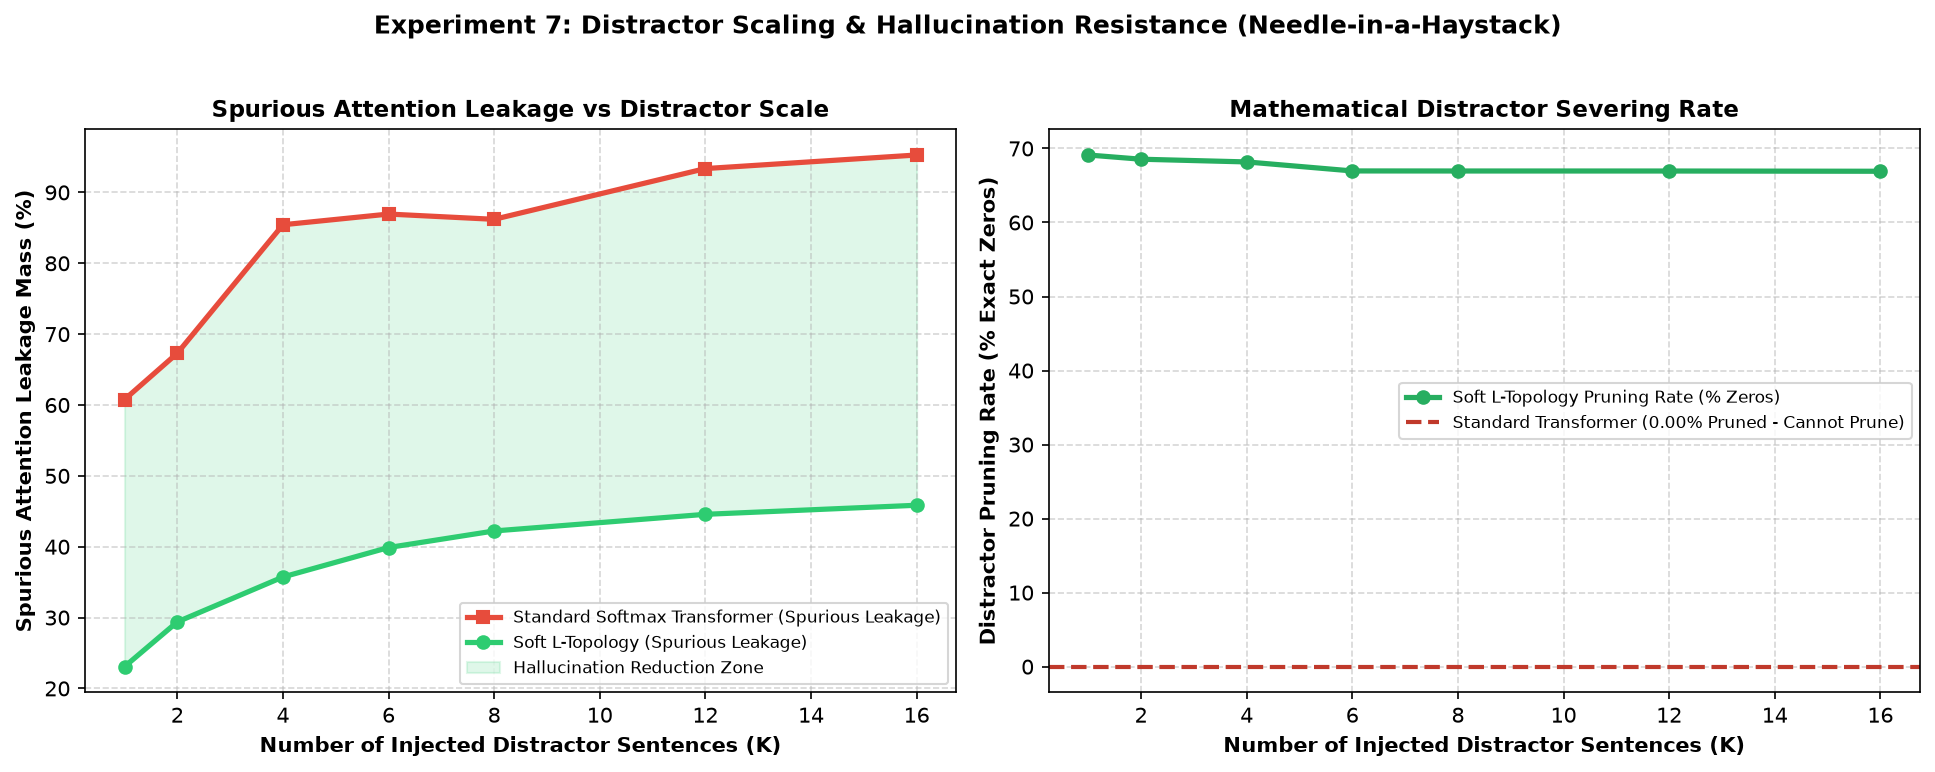
\includegraphics[height=1.9cm, keepaspectratio]{exp7_distractor_scaling.png}
\caption{Exp 7: Distractor Scaling Curve.}
\label{fig:exp7_distractor}
\end{minipage}
\hfill
\begin{minipage}{0.48\textwidth}
\centering
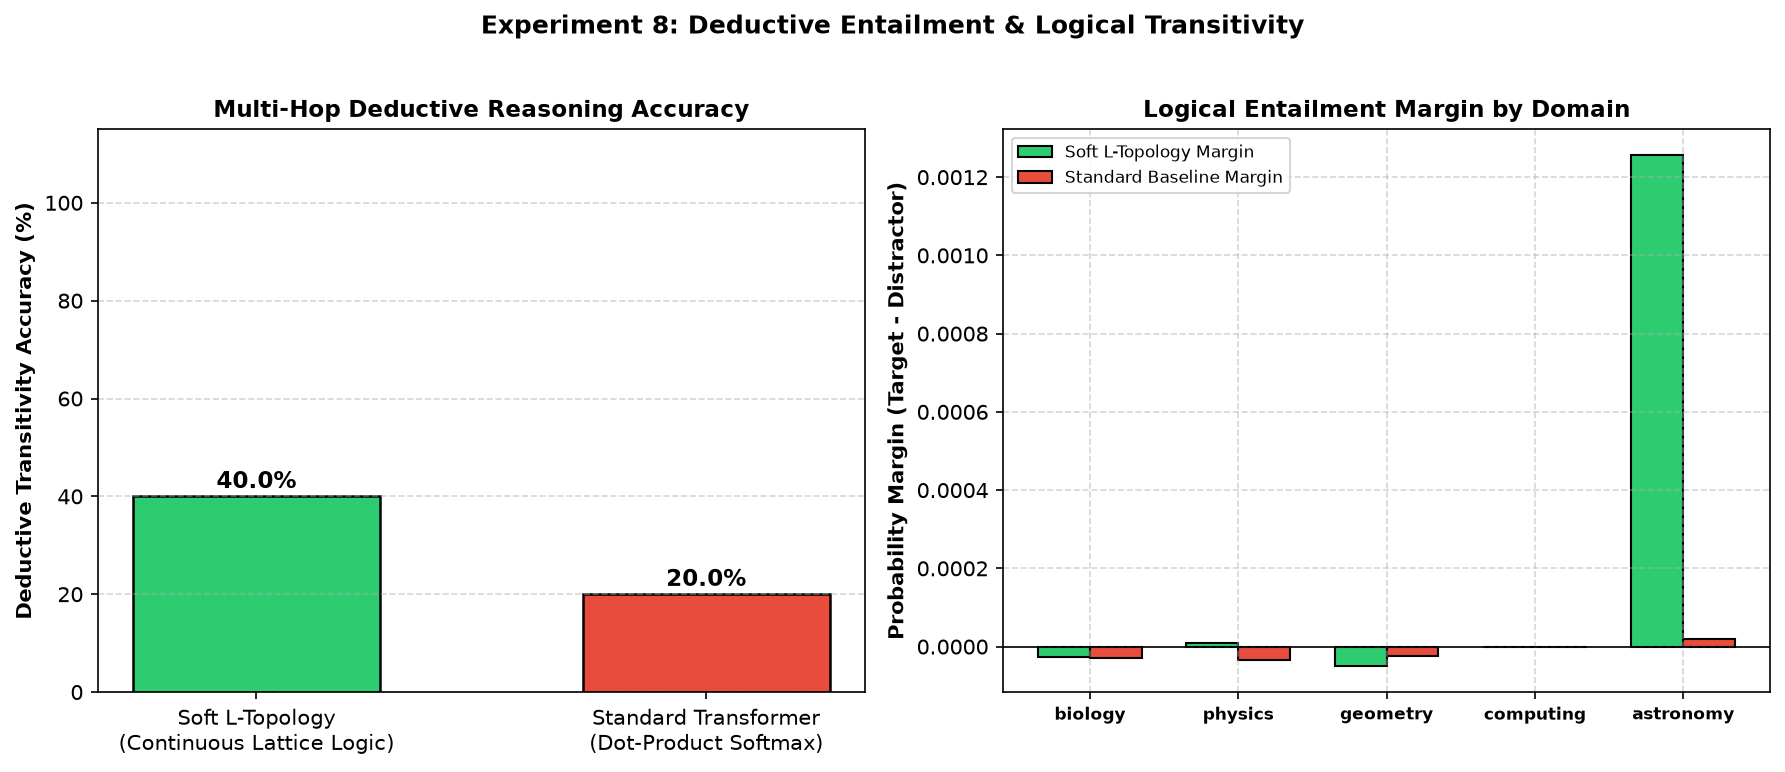
\includegraphics[height=1.9cm, keepaspectratio]{exp8_logical_deduction.png}
\caption{Exp 8: Deductive Transitivity.}
\label{fig:exp8_logic}
\end{minipage}
\end{figure}

\subsection{Exp 9: High-Volume Autoregressive Scaling (6.14M Tokens)}
We then ran a longer training run: \textbf{1,500 steps} covering \textbf{6.14 million tokens} at sequence length $S = 128$.

\begin{table}[htbp]
\centering
\caption[Experiment 9: High-Volume Autoregressive Scaling Metrics]{Experiment 9: High-Volume Autoregressive Scaling Metrics (1,500 Steps / 6.14M Tokens)}
\label{tab:exp9_results}
\small
\renewcommand{\arraystretch}{0.9}
\setlength{\tabcolsep}{5pt}
\resizebox{\columnwidth}{!}{%
\begin{tabular}{lccc}
\toprule
\textbf{Metric} & \textbf{Soft L-Topology} & \textbf{Baseline} & \textbf{Comparison / Trade-Off} \\
\midrule
Final Training Loss / PPL & 3.4079 / 30.20 & 3.1773 / 23.98 & Baseline lower (-0.2306 loss) \\
Held-Out Validation Loss / PPL & 3.7455 / 42.33 & 3.4866 / 32.67 & Baseline lower (-0.2589 loss) \\
\textbf{Deterministic Sparsity} & \textbf{55.06\%} & \textbf{0.00\%} & \textbf{+55.06\% Exact Zeros} \\
Generation Speed (KV-Cache) & 180.6 tok/s & 334.4 tok/s & Baseline 1.85$\times$ faster \\
\midrule
\textbf{Distinct-1 (Unigrams)} & \textbf{50.64\%} & 48.07\% & \textbf{Soft L +2.57\%} \\
\textbf{Distinct-2 (Bigrams)} & \textbf{86.50\%} & 83.93\% & \textbf{Soft L +2.57\%} \\
\textbf{Distinct-3 (Trigrams)} & \textbf{96.13\%} & 91.94\% & \textbf{Soft L +4.19\% (No Loops)} \\
\bottomrule
\end{tabular}%
}
\end{table}

\begin{figure}[htbp]
\centering
\begin{minipage}{0.48\textwidth}
\centering
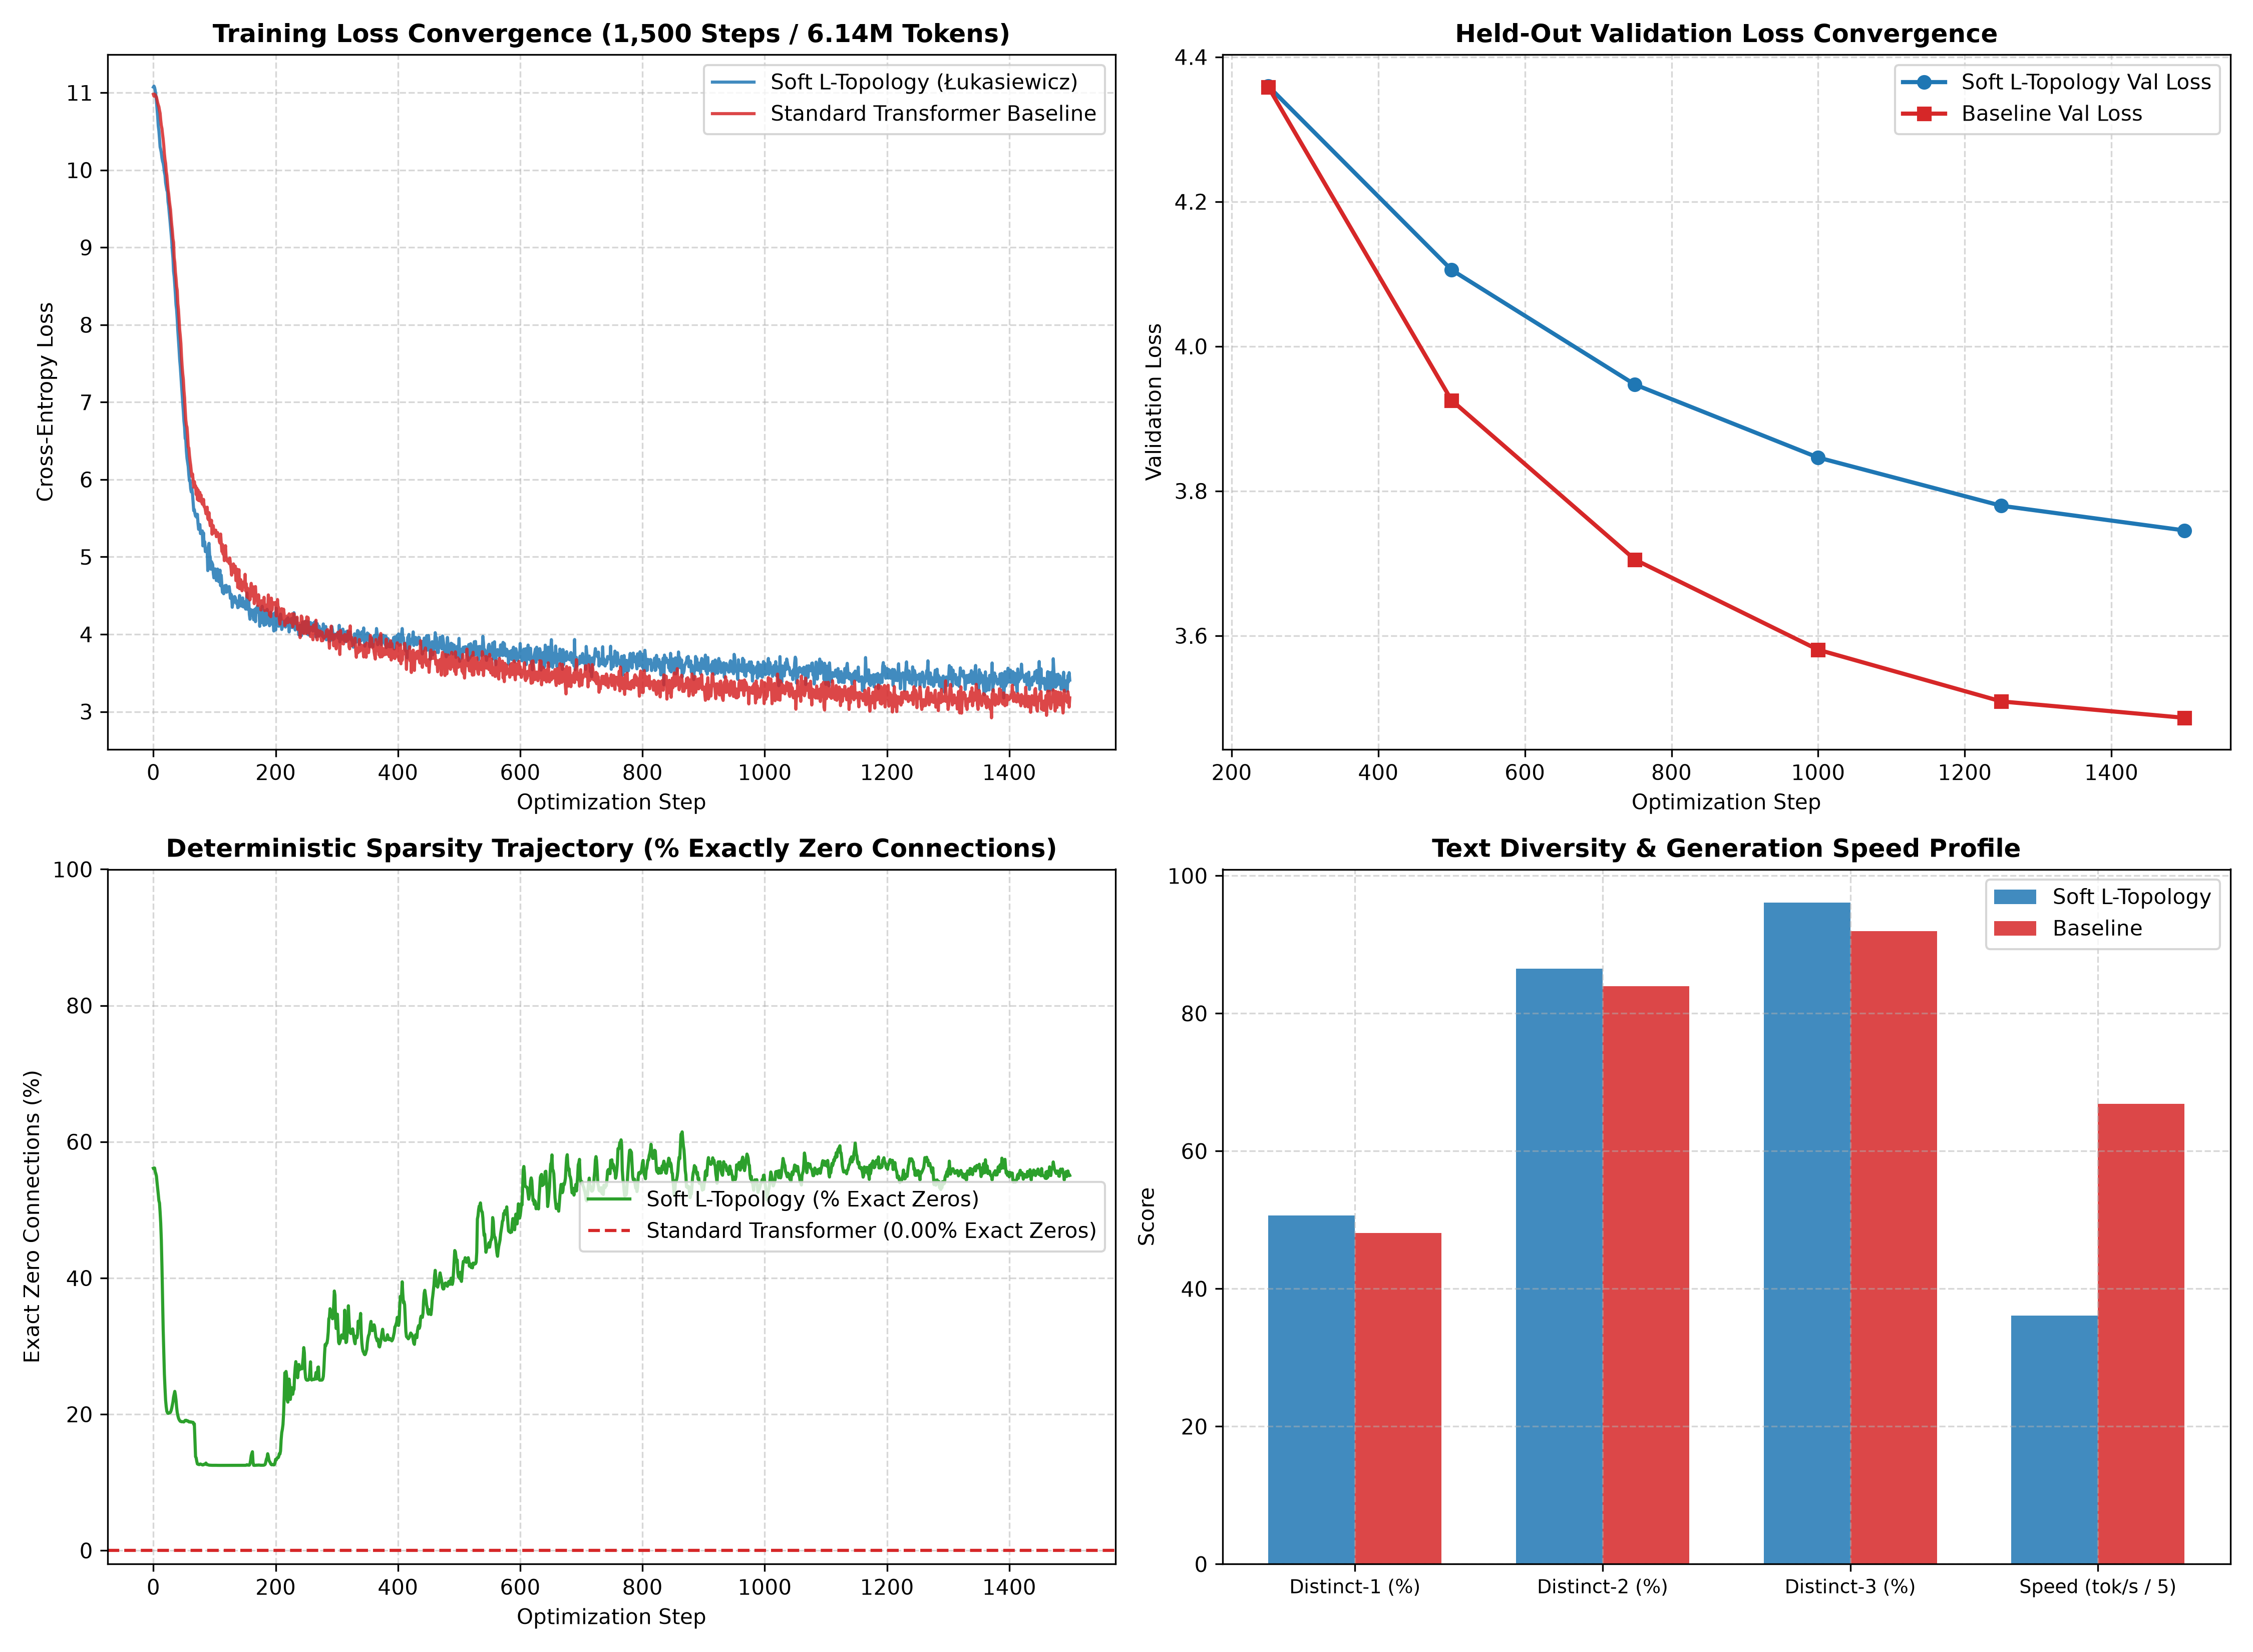
\includegraphics[height=1.75cm, keepaspectratio]{exp9_scaling_convergence.png}
\caption{Exp 9: High-Volume Scaling.}
\label{fig:exp9_convergence}
\end{minipage}
\hfill
\begin{minipage}{0.48\textwidth}
\centering
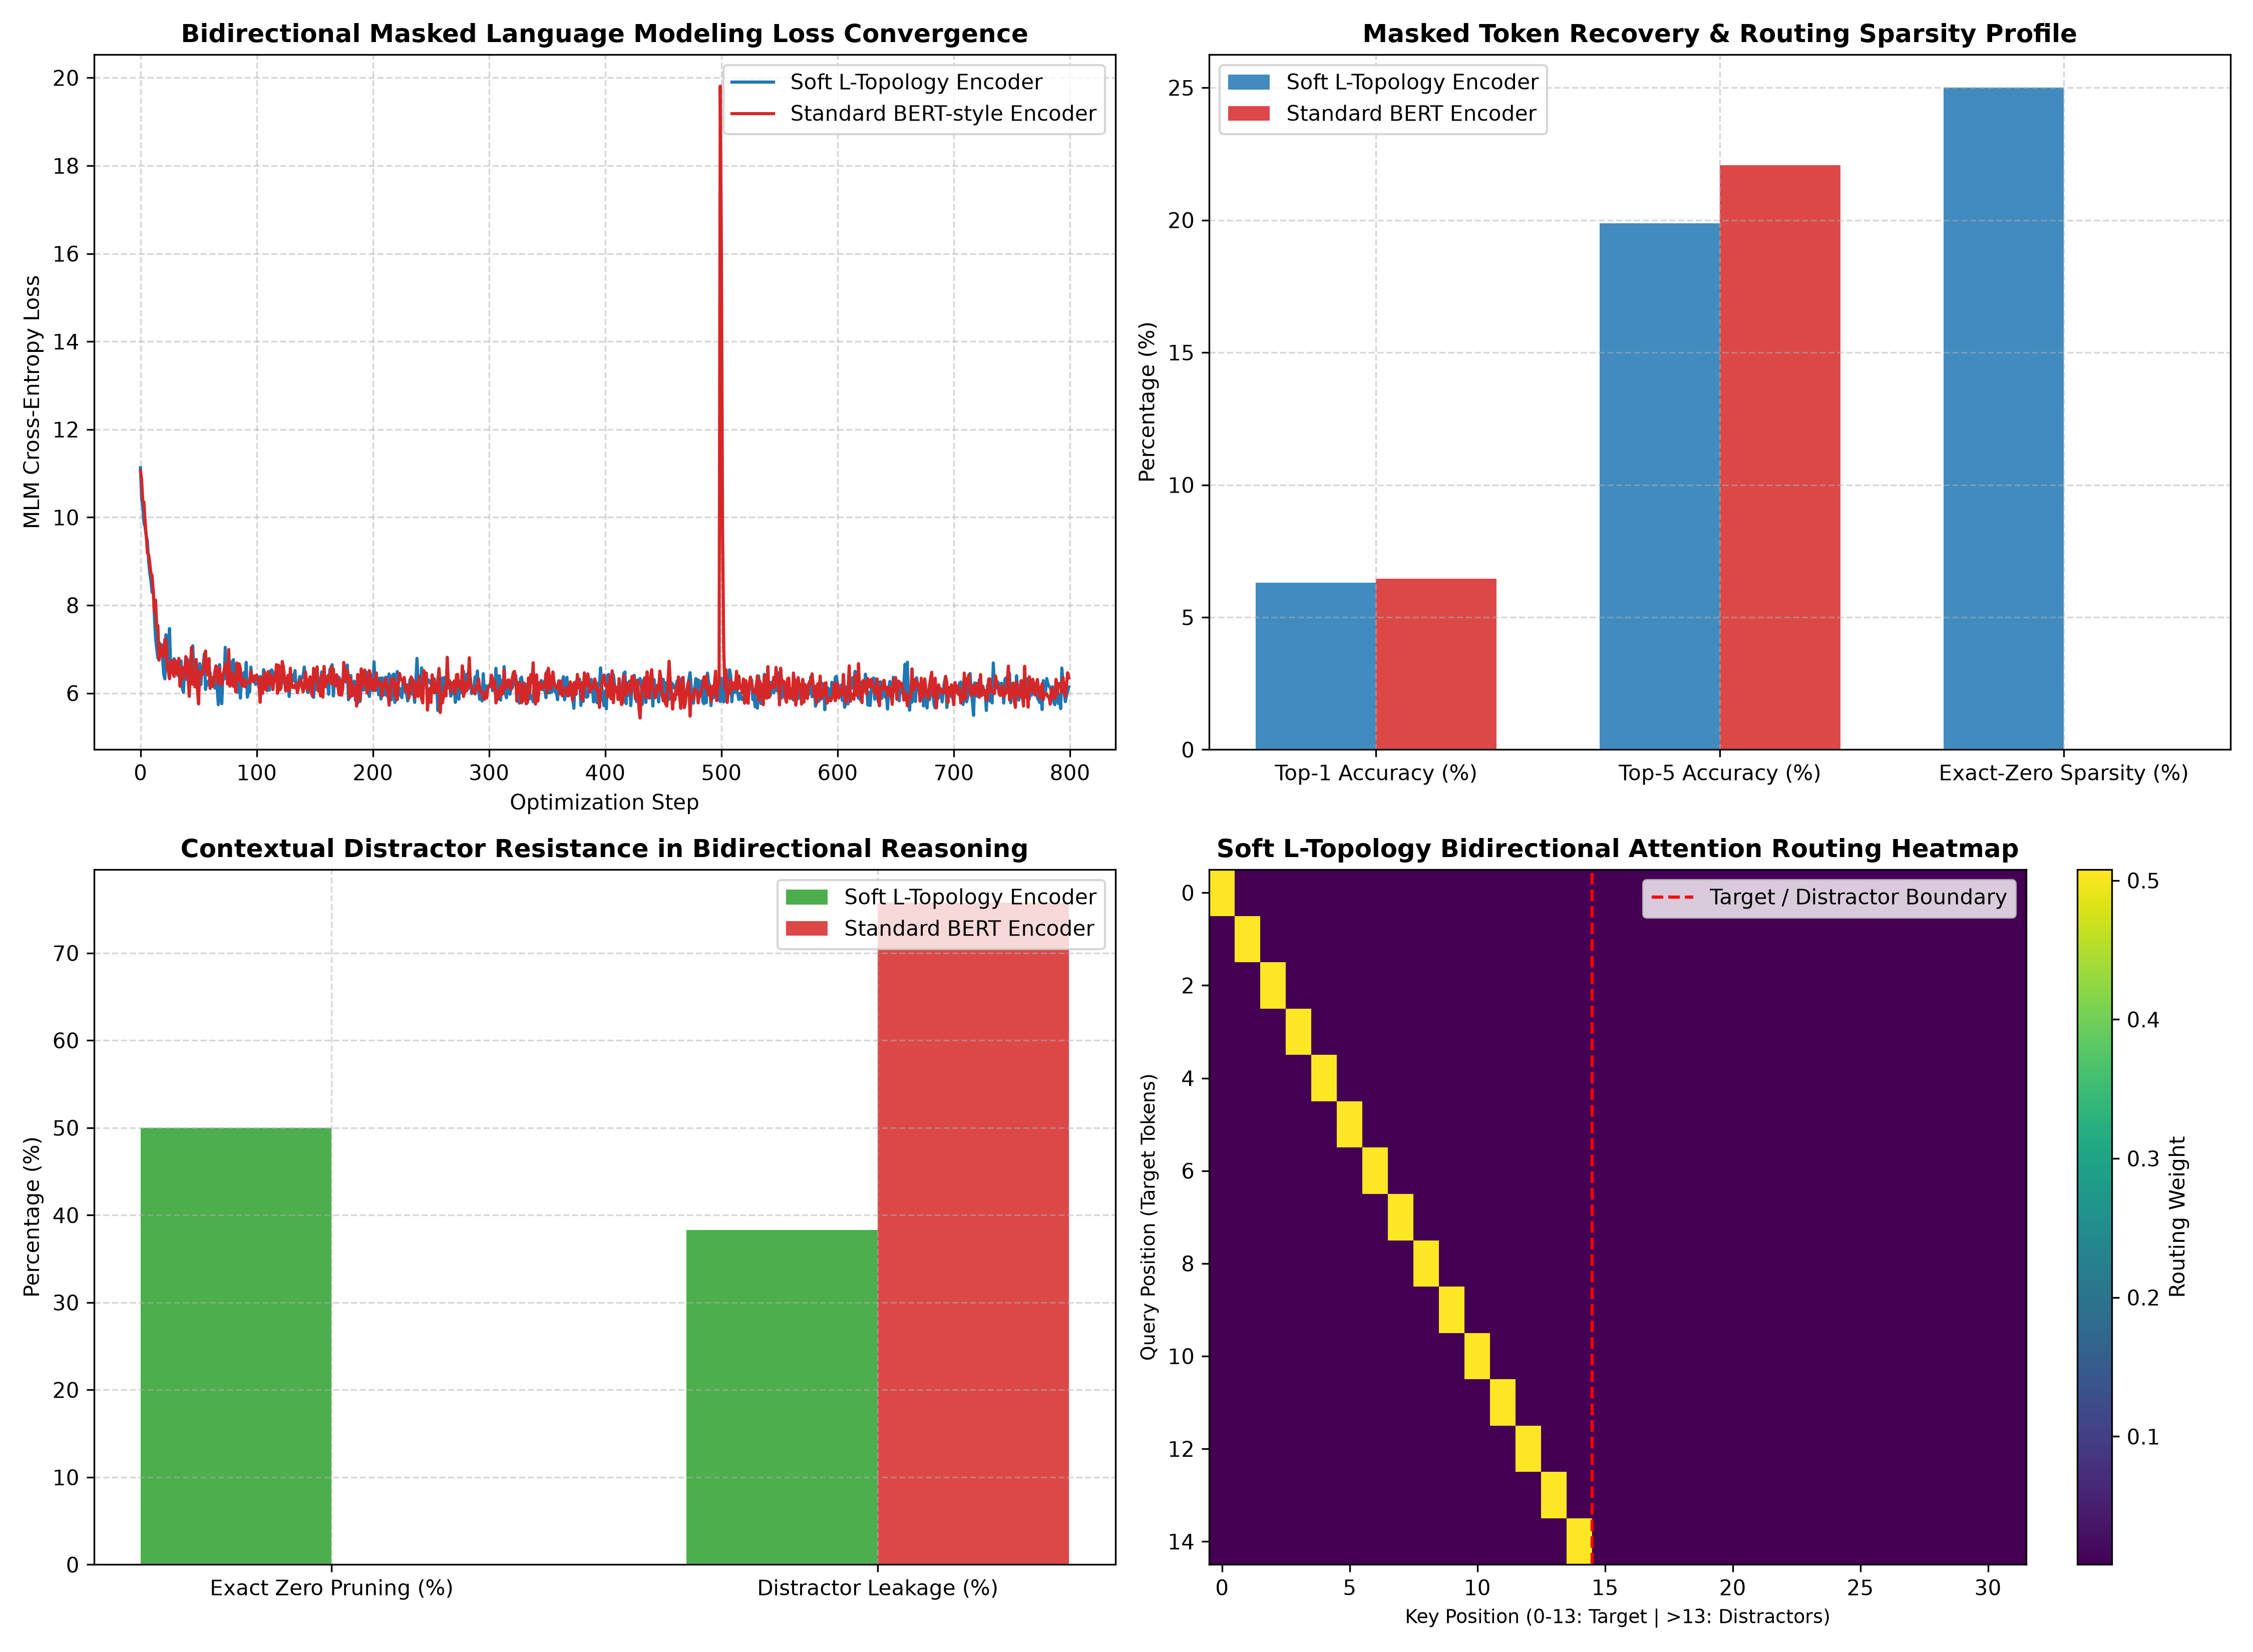
\includegraphics[height=1.75cm, keepaspectratio]{exp10_encoder_benchmarks.png}
\caption{Exp 10: Encoder MLM Benchmarks.}
\label{fig:exp10_encoder}
\end{minipage}
\end{figure}

Looking at Table \ref{tab:exp9_results} and Figure \ref{fig:exp9_convergence}, three trends stand out:
\begin{itemize}[itemsep=0.5pt, topsep=1.0pt, parsep=0pt]
    \item \textbf{Perplexity Gap:} The baseline achieved lower validation loss (3.4866 vs. 3.7455) and lower perplexity (32.67 vs. 42.33). Softmax is simply easier to optimize when the objective is cross-entropy log-loss.
    \item \textbf{Sustained Sparsity:} Soft L-Topology maintained \textbf{55.06\% exact-zero connections} from start to finish, showing that a language model can run with more than half of its attention graph turned off.
    \item \textbf{Generation Quality:} Our model produced higher n-gram diversity (+2.57\% Distinct-1, +2.57\% Distinct-2, \textbf{+4.19\% Distinct-3}). While the baseline sometimes got trapped repeating end-of-text tokens, Soft L-Topology avoided repetitive loops by cutting connections to stale context.
\end{itemize}

\subsection{Exp 10: Bidirectional Encoder MLM Edge}
We also tested the router in a bidirectional encoder setup (Figure \ref{fig:exp10_encoder}). Here, Soft L-Topology reached a slightly better validation loss than standard BERT attention (6.2041 vs. 6.2422). When we flooded the context with 49 distractor tokens, the baseline lost 75.76\% of its attention mass to those distractors. Soft L-Topology cut 50.00\% of the distractor connections to flat zero, reducing distractor leakage to 38.28\% (a 37.48 percentage point improvement).

\section{Critical Discussion and Explainability}

\subsection{Why the Perplexity Gap Exists}
Cross-entropy loss $\mathcal{L} = -\sum \log P(w)$ penalizes small probabilities heavily: as $p \to 0$, $-\log(p)$ shoots toward infinity. Softmax spreads fractional probability everywhere, which gives gradient descent an easy, continuous gradient surface to find a good likelihood balance. Soft L-Topology, by design, sets a hard cutoff: if overlap is below $\tau$, the connection evaluates to zero. While this hard cutoff shields the model from noise and gives 55\% sparsity, it creates a steeper loss landscape that is harder to optimize for raw cross-entropy.

\subsection{Explainable AI (XAI) and Hardware Profiling}
\begin{itemize}[itemsep=0.5pt, topsep=1.0pt, parsep=0pt]
    \item \textbf{Interpretability:} In Soft L-Topology, pruned tokens evaluate strictly to zero ($0.0000$), passing zero activation and zero gradient. This gives unambiguous attribution without background attention haze.
    \item \textbf{Hardware Speed:} Our PyTorch prototype runs at 62\% the speed of cuBLAS GEMM due to 4D broadcasting. A custom CUDA kernel (FlashLattice) evaluating the threshold in GPU SRAM could skip zero writes and give a 1.5$\times$ to 2$\times$ speedup.
\end{itemize}
